% Options for packages loaded elsewhere
\PassOptionsToPackage{unicode}{hyperref}
\PassOptionsToPackage{hyphens}{url}
\PassOptionsToPackage{dvipsnames,svgnames,x11names}{xcolor}
%
\documentclass[
  letterpaper,
  DIV=11,
  numbers=noendperiod]{scrartcl}

\usepackage{amsmath,amssymb}
\usepackage{iftex}
\ifPDFTeX
  \usepackage[T1]{fontenc}
  \usepackage[utf8]{inputenc}
  \usepackage{textcomp} % provide euro and other symbols
\else % if luatex or xetex
  \usepackage{unicode-math}
  \defaultfontfeatures{Scale=MatchLowercase}
  \defaultfontfeatures[\rmfamily]{Ligatures=TeX,Scale=1}
\fi
\usepackage{lmodern}
\ifPDFTeX\else  
    % xetex/luatex font selection
\fi
% Use upquote if available, for straight quotes in verbatim environments
\IfFileExists{upquote.sty}{\usepackage{upquote}}{}
\IfFileExists{microtype.sty}{% use microtype if available
  \usepackage[]{microtype}
  \UseMicrotypeSet[protrusion]{basicmath} % disable protrusion for tt fonts
}{}
\makeatletter
\@ifundefined{KOMAClassName}{% if non-KOMA class
  \IfFileExists{parskip.sty}{%
    \usepackage{parskip}
  }{% else
    \setlength{\parindent}{0pt}
    \setlength{\parskip}{6pt plus 2pt minus 1pt}}
}{% if KOMA class
  \KOMAoptions{parskip=half}}
\makeatother
\usepackage{xcolor}
\setlength{\emergencystretch}{3em} % prevent overfull lines
\setcounter{secnumdepth}{-\maxdimen} % remove section numbering
% Make \paragraph and \subparagraph free-standing
\ifx\paragraph\undefined\else
  \let\oldparagraph\paragraph
  \renewcommand{\paragraph}[1]{\oldparagraph{#1}\mbox{}}
\fi
\ifx\subparagraph\undefined\else
  \let\oldsubparagraph\subparagraph
  \renewcommand{\subparagraph}[1]{\oldsubparagraph{#1}\mbox{}}
\fi

\usepackage{color}
\usepackage{fancyvrb}
\newcommand{\VerbBar}{|}
\newcommand{\VERB}{\Verb[commandchars=\\\{\}]}
\DefineVerbatimEnvironment{Highlighting}{Verbatim}{commandchars=\\\{\}}
% Add ',fontsize=\small' for more characters per line
\usepackage{framed}
\definecolor{shadecolor}{RGB}{241,243,245}
\newenvironment{Shaded}{\begin{snugshade}}{\end{snugshade}}
\newcommand{\AlertTok}[1]{\textcolor[rgb]{0.68,0.00,0.00}{#1}}
\newcommand{\AnnotationTok}[1]{\textcolor[rgb]{0.37,0.37,0.37}{#1}}
\newcommand{\AttributeTok}[1]{\textcolor[rgb]{0.40,0.45,0.13}{#1}}
\newcommand{\BaseNTok}[1]{\textcolor[rgb]{0.68,0.00,0.00}{#1}}
\newcommand{\BuiltInTok}[1]{\textcolor[rgb]{0.00,0.23,0.31}{#1}}
\newcommand{\CharTok}[1]{\textcolor[rgb]{0.13,0.47,0.30}{#1}}
\newcommand{\CommentTok}[1]{\textcolor[rgb]{0.37,0.37,0.37}{#1}}
\newcommand{\CommentVarTok}[1]{\textcolor[rgb]{0.37,0.37,0.37}{\textit{#1}}}
\newcommand{\ConstantTok}[1]{\textcolor[rgb]{0.56,0.35,0.01}{#1}}
\newcommand{\ControlFlowTok}[1]{\textcolor[rgb]{0.00,0.23,0.31}{#1}}
\newcommand{\DataTypeTok}[1]{\textcolor[rgb]{0.68,0.00,0.00}{#1}}
\newcommand{\DecValTok}[1]{\textcolor[rgb]{0.68,0.00,0.00}{#1}}
\newcommand{\DocumentationTok}[1]{\textcolor[rgb]{0.37,0.37,0.37}{\textit{#1}}}
\newcommand{\ErrorTok}[1]{\textcolor[rgb]{0.68,0.00,0.00}{#1}}
\newcommand{\ExtensionTok}[1]{\textcolor[rgb]{0.00,0.23,0.31}{#1}}
\newcommand{\FloatTok}[1]{\textcolor[rgb]{0.68,0.00,0.00}{#1}}
\newcommand{\FunctionTok}[1]{\textcolor[rgb]{0.28,0.35,0.67}{#1}}
\newcommand{\ImportTok}[1]{\textcolor[rgb]{0.00,0.46,0.62}{#1}}
\newcommand{\InformationTok}[1]{\textcolor[rgb]{0.37,0.37,0.37}{#1}}
\newcommand{\KeywordTok}[1]{\textcolor[rgb]{0.00,0.23,0.31}{#1}}
\newcommand{\NormalTok}[1]{\textcolor[rgb]{0.00,0.23,0.31}{#1}}
\newcommand{\OperatorTok}[1]{\textcolor[rgb]{0.37,0.37,0.37}{#1}}
\newcommand{\OtherTok}[1]{\textcolor[rgb]{0.00,0.23,0.31}{#1}}
\newcommand{\PreprocessorTok}[1]{\textcolor[rgb]{0.68,0.00,0.00}{#1}}
\newcommand{\RegionMarkerTok}[1]{\textcolor[rgb]{0.00,0.23,0.31}{#1}}
\newcommand{\SpecialCharTok}[1]{\textcolor[rgb]{0.37,0.37,0.37}{#1}}
\newcommand{\SpecialStringTok}[1]{\textcolor[rgb]{0.13,0.47,0.30}{#1}}
\newcommand{\StringTok}[1]{\textcolor[rgb]{0.13,0.47,0.30}{#1}}
\newcommand{\VariableTok}[1]{\textcolor[rgb]{0.07,0.07,0.07}{#1}}
\newcommand{\VerbatimStringTok}[1]{\textcolor[rgb]{0.13,0.47,0.30}{#1}}
\newcommand{\WarningTok}[1]{\textcolor[rgb]{0.37,0.37,0.37}{\textit{#1}}}

\providecommand{\tightlist}{%
  \setlength{\itemsep}{0pt}\setlength{\parskip}{0pt}}\usepackage{longtable,booktabs,array}
\usepackage{calc} % for calculating minipage widths
% Correct order of tables after \paragraph or \subparagraph
\usepackage{etoolbox}
\makeatletter
\patchcmd\longtable{\par}{\if@noskipsec\mbox{}\fi\par}{}{}
\makeatother
% Allow footnotes in longtable head/foot
\IfFileExists{footnotehyper.sty}{\usepackage{footnotehyper}}{\usepackage{footnote}}
\makesavenoteenv{longtable}
\usepackage{graphicx}
\makeatletter
\def\maxwidth{\ifdim\Gin@nat@width>\linewidth\linewidth\else\Gin@nat@width\fi}
\def\maxheight{\ifdim\Gin@nat@height>\textheight\textheight\else\Gin@nat@height\fi}
\makeatother
% Scale images if necessary, so that they will not overflow the page
% margins by default, and it is still possible to overwrite the defaults
% using explicit options in \includegraphics[width, height, ...]{}
\setkeys{Gin}{width=\maxwidth,height=\maxheight,keepaspectratio}
% Set default figure placement to htbp
\makeatletter
\def\fps@figure{htbp}
\makeatother

\KOMAoption{captions}{tableheading}
\makeatletter
\@ifpackageloaded{tcolorbox}{}{\usepackage[skins,breakable]{tcolorbox}}
\@ifpackageloaded{fontawesome5}{}{\usepackage{fontawesome5}}
\definecolor{quarto-callout-color}{HTML}{909090}
\definecolor{quarto-callout-note-color}{HTML}{0758E5}
\definecolor{quarto-callout-important-color}{HTML}{CC1914}
\definecolor{quarto-callout-warning-color}{HTML}{EB9113}
\definecolor{quarto-callout-tip-color}{HTML}{00A047}
\definecolor{quarto-callout-caution-color}{HTML}{FC5300}
\definecolor{quarto-callout-color-frame}{HTML}{acacac}
\definecolor{quarto-callout-note-color-frame}{HTML}{4582ec}
\definecolor{quarto-callout-important-color-frame}{HTML}{d9534f}
\definecolor{quarto-callout-warning-color-frame}{HTML}{f0ad4e}
\definecolor{quarto-callout-tip-color-frame}{HTML}{02b875}
\definecolor{quarto-callout-caution-color-frame}{HTML}{fd7e14}
\makeatother
\makeatletter
\@ifpackageloaded{caption}{}{\usepackage{caption}}
\AtBeginDocument{%
\ifdefined\contentsname
  \renewcommand*\contentsname{Table of contents}
\else
  \newcommand\contentsname{Table of contents}
\fi
\ifdefined\listfigurename
  \renewcommand*\listfigurename{List of Figures}
\else
  \newcommand\listfigurename{List of Figures}
\fi
\ifdefined\listtablename
  \renewcommand*\listtablename{List of Tables}
\else
  \newcommand\listtablename{List of Tables}
\fi
\ifdefined\figurename
  \renewcommand*\figurename{Figure}
\else
  \newcommand\figurename{Figure}
\fi
\ifdefined\tablename
  \renewcommand*\tablename{Table}
\else
  \newcommand\tablename{Table}
\fi
}
\@ifpackageloaded{float}{}{\usepackage{float}}
\floatstyle{ruled}
\@ifundefined{c@chapter}{\newfloat{codelisting}{h}{lop}}{\newfloat{codelisting}{h}{lop}[chapter]}
\floatname{codelisting}{Listing}
\newcommand*\listoflistings{\listof{codelisting}{List of Listings}}
\makeatother
\makeatletter
\makeatother
\makeatletter
\@ifpackageloaded{caption}{}{\usepackage{caption}}
\@ifpackageloaded{subcaption}{}{\usepackage{subcaption}}
\makeatother
\ifLuaTeX
  \usepackage{selnolig}  % disable illegal ligatures
\fi
\usepackage{bookmark}

\IfFileExists{xurl.sty}{\usepackage{xurl}}{} % add URL line breaks if available
\urlstyle{same} % disable monospaced font for URLs
\hypersetup{
  pdftitle={인공지능 및 기계학습 과제1},
  colorlinks=true,
  linkcolor={blue},
  filecolor={Maroon},
  citecolor={Blue},
  urlcolor={Blue},
  pdfcreator={LaTeX via pandoc}}

\title{인공지능 및 기계학습 과제1}
\author{}
\date{}

\begin{document}
\maketitle

20249132 김형환

\subsection{Question 1}\label{question-1}

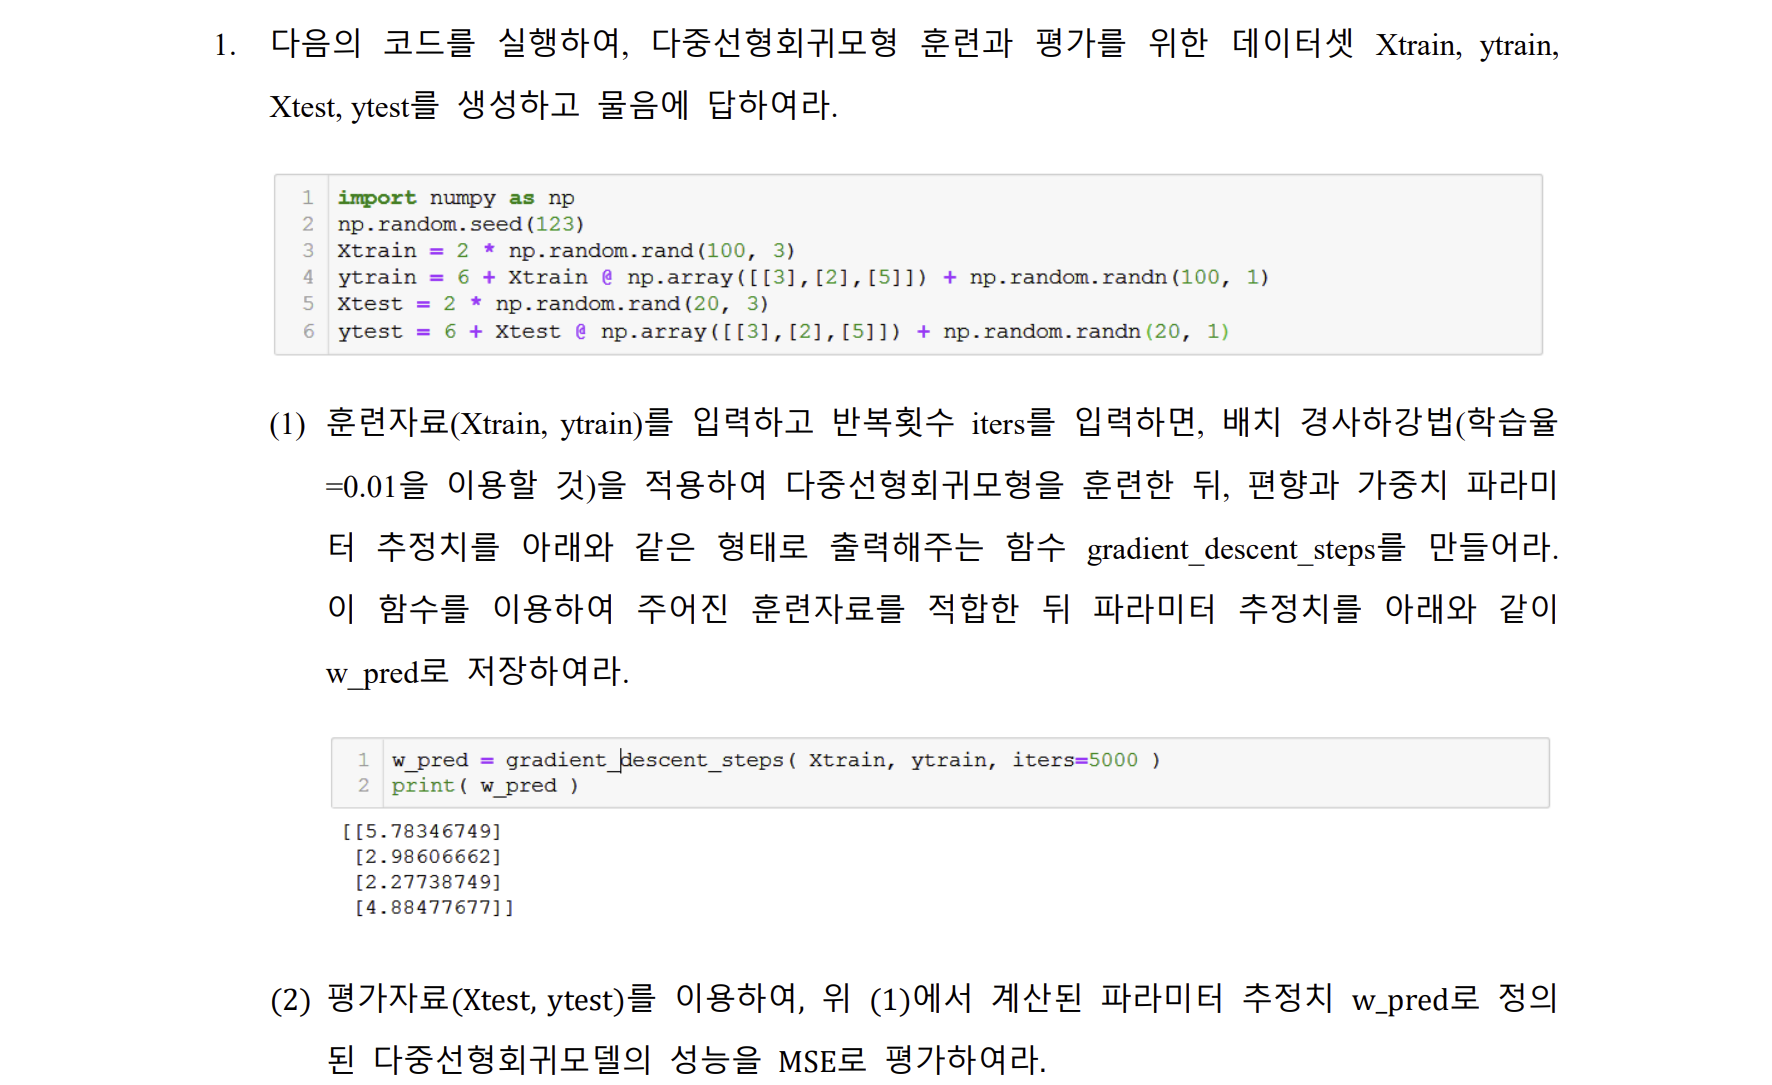
\includegraphics{image/machine_hw1_1.png}

\subsubsection{Answer}\label{answer}

\begin{Shaded}
\begin{Highlighting}[]
\ImportTok{import}\NormalTok{ numpy }\ImportTok{as}\NormalTok{ np}
\ImportTok{from}\NormalTok{ sklearn.metrics }\ImportTok{import}\NormalTok{ mean\_squared\_error}

\NormalTok{np.random.seed(}\DecValTok{123}\NormalTok{)}
\NormalTok{xtrain }\OperatorTok{=} \DecValTok{2} \OperatorTok{*}\NormalTok{ np.random.rand(}\DecValTok{100}\NormalTok{, }\DecValTok{3}\NormalTok{)}
\NormalTok{ytrain }\OperatorTok{=} \DecValTok{6} \OperatorTok{+}\NormalTok{ xtrain }\OperatorTok{@}\NormalTok{ np.array([[}\DecValTok{3}\NormalTok{],[}\DecValTok{2}\NormalTok{],[}\DecValTok{5}\NormalTok{]]) }\OperatorTok{+}\NormalTok{ np.random.randn(}\DecValTok{100}\NormalTok{, }\DecValTok{1}\NormalTok{)}
\NormalTok{xtest }\OperatorTok{=} \DecValTok{2} \OperatorTok{*}\NormalTok{ np.random.rand(}\DecValTok{20}\NormalTok{, }\DecValTok{3}\NormalTok{)}
\NormalTok{ytest }\OperatorTok{=} \DecValTok{6} \OperatorTok{+}\NormalTok{ xtest }\OperatorTok{@}\NormalTok{ np.array([[}\DecValTok{3}\NormalTok{],[}\DecValTok{2}\NormalTok{],[}\DecValTok{5}\NormalTok{]]) }\OperatorTok{+}\NormalTok{ np.random.randn(}\DecValTok{20}\NormalTok{,}\DecValTok{1}\NormalTok{)}

\CommentTok{\# (1)}
\KeywordTok{def}\NormalTok{ gradient\_descent\_steps(xtrain, ytrain, iters):}
    \CommentTok{\# m = 훈련데이터의 수, n = 변수의 개수}
\NormalTok{    m, n }\OperatorTok{=}\NormalTok{ xtrain.shape}
    \CommentTok{\# 절편항 추가를 위해 x0=1을 각 훈련데이터에 추가}
\NormalTok{    X }\OperatorTok{=}\NormalTok{ np.insert(xtrain, }\DecValTok{0}\NormalTok{, }\DecValTok{1}\NormalTok{, axis }\OperatorTok{=} \DecValTok{1}\NormalTok{)}
\NormalTok{    Y }\OperatorTok{=}\NormalTok{ ytrain}
    \CommentTok{\# 파라미터 theta의 초기값은 1, 절편항까지 n+1개 }
\NormalTok{    theta }\OperatorTok{=}\NormalTok{ np.ones(n}\OperatorTok{+}\DecValTok{1}\NormalTok{).reshape(n}\OperatorTok{+}\DecValTok{1}\NormalTok{,}\DecValTok{1}\NormalTok{)}
    \ControlFlowTok{for}\NormalTok{ i }\KeywordTok{in} \BuiltInTok{range}\NormalTok{(iters):}
        \CommentTok{\# 비용함수 = (오차의 제곱합) / 2m 형태로 가정 }
\NormalTok{        gradient }\OperatorTok{=}\NormalTok{ X.T }\OperatorTok{@}\NormalTok{ (X }\OperatorTok{@}\NormalTok{ theta }\OperatorTok{{-}}\NormalTok{ Y) }\OperatorTok{/}\NormalTok{ m}
\NormalTok{        theta }\OperatorTok{{-}=}\FloatTok{0.01} \OperatorTok{*}\NormalTok{ gradient}
    \ControlFlowTok{return}\NormalTok{ theta}

\NormalTok{w\_pred }\OperatorTok{=}\NormalTok{ gradient\_descent\_steps(xtrain, ytrain, iters}\OperatorTok{=}\DecValTok{5000}\NormalTok{)}
\BuiltInTok{print}\NormalTok{(}\StringTok{"Best parameters are :"}\NormalTok{)}
\BuiltInTok{print}\NormalTok{( w\_pred )}

\CommentTok{\# (2)}
\NormalTok{ypred }\OperatorTok{=}\NormalTok{ np.insert(xtest,}\DecValTok{0}\NormalTok{,}\DecValTok{1}\NormalTok{,axis }\OperatorTok{=} \DecValTok{1}\NormalTok{) }\OperatorTok{@}\NormalTok{ w\_pred}
\NormalTok{mse }\OperatorTok{=}\NormalTok{ mean\_squared\_error(ypred, ytest)}
\BuiltInTok{print}\NormalTok{(}\StringTok{"Mean Squared Error is :"}\NormalTok{)}
\BuiltInTok{print}\NormalTok{(mse)}
\end{Highlighting}
\end{Shaded}

\begin{verbatim}
Best parameters are :
[[5.72120369]
 [3.00637126]
 [2.29860859]
 [4.9014743 ]]
Mean Squared Error is :
0.8604989666540144
\end{verbatim}

\subsection{Question 2}\label{question-2}

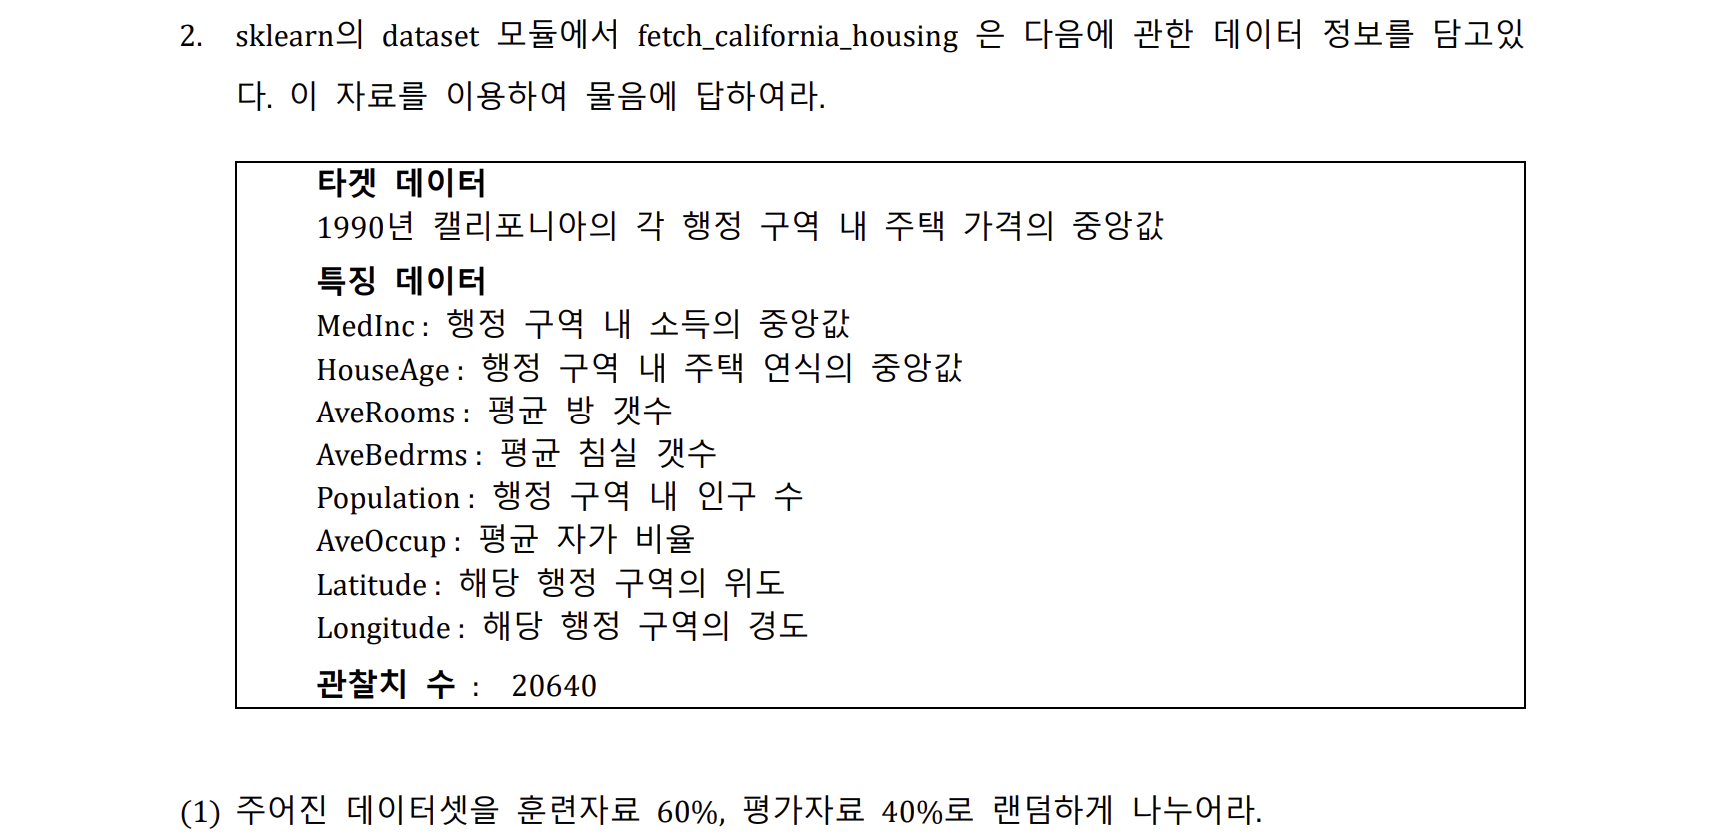
\includegraphics{image/machine_hw1_2.png}

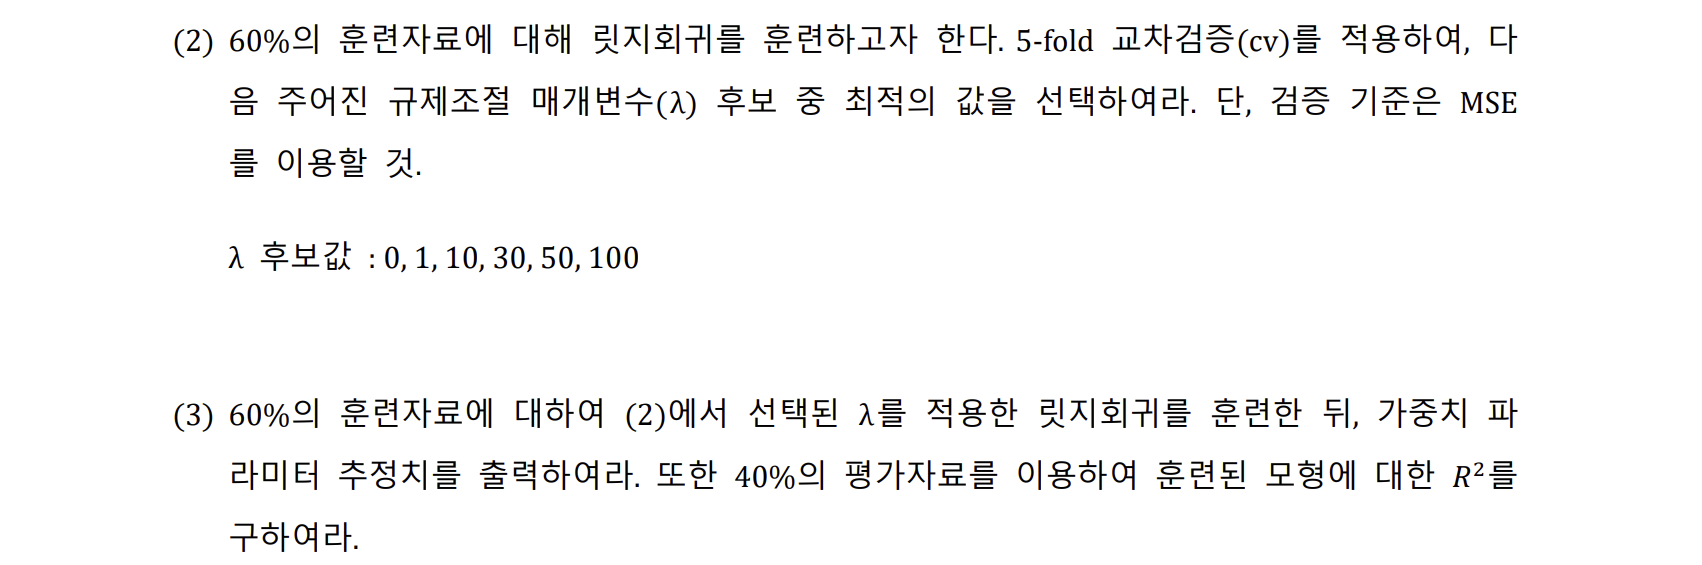
\includegraphics{image/machine_hw1_3.png}

\begin{Shaded}
\begin{Highlighting}[]
\ImportTok{import}\NormalTok{ pandas }\ImportTok{as}\NormalTok{ pd}
\ImportTok{from}\NormalTok{ sklearn.datasets }\ImportTok{import}\NormalTok{ fetch\_california\_housing}
\ImportTok{from}\NormalTok{ sklearn.model\_selection }\ImportTok{import}\NormalTok{ train\_test\_split}

\NormalTok{housing }\OperatorTok{=}\NormalTok{ fetch\_california\_housing()}

\CommentTok{\# (1)}
\NormalTok{y }\OperatorTok{=}\NormalTok{ housing[}\StringTok{\textquotesingle{}target\textquotesingle{}}\NormalTok{]}
\NormalTok{x }\OperatorTok{=}\NormalTok{ pd.DataFrame( housing[}\StringTok{\textquotesingle{}data\textquotesingle{}}\NormalTok{], columns}\OperatorTok{=}\NormalTok{housing[}\StringTok{\textquotesingle{}feature\_names\textquotesingle{}}\NormalTok{] )}

\CommentTok{\# train\_test\_split 모듈 이용}
\NormalTok{x\_train, x\_test, y\_train, y\_test }\OperatorTok{=}\NormalTok{ train\_test\_split(x,y,test\_size}\OperatorTok{=}\FloatTok{0.4}\NormalTok{)}
\BuiltInTok{print}\NormalTok{(}\StringTok{"Split data to training 0.6 and test 0.4 ratio"}\NormalTok{)}
\BuiltInTok{print}\NormalTok{(}\StringTok{"Data size of X train, test : "}\NormalTok{,x\_train.shape[}\DecValTok{0}\NormalTok{], x\_test.shape[}\DecValTok{0}\NormalTok{])}
\BuiltInTok{print}\NormalTok{(}\StringTok{"Data size of y train, test : "}\NormalTok{,y\_train.shape[}\DecValTok{0}\NormalTok{], y\_test.shape[}\DecValTok{0}\NormalTok{])}
\end{Highlighting}
\end{Shaded}

\begin{verbatim}
Split data to training 0.6 and test 0.4 ratio
Data size of X train, test :  12384 8256
Data size of y train, test :  12384 8256
\end{verbatim}

\begin{Shaded}
\begin{Highlighting}[]
\ImportTok{from}\NormalTok{ sklearn.linear\_model }\ImportTok{import}\NormalTok{ Ridge}
\ImportTok{from}\NormalTok{ sklearn.model\_selection }\ImportTok{import}\NormalTok{ GridSearchCV}

\CommentTok{\# (2) GridSearchCV 모듈 활용. 하이퍼파라미터 튜닝 및 재훈련.}
\NormalTok{params }\OperatorTok{=}\NormalTok{ \{}\StringTok{\textquotesingle{}alpha\textquotesingle{}}\NormalTok{: [}\DecValTok{0}\NormalTok{, }\DecValTok{1}\NormalTok{, }\DecValTok{10}\NormalTok{, }\DecValTok{30}\NormalTok{, }\DecValTok{50}\NormalTok{, }\DecValTok{100}\NormalTok{]\}}
\NormalTok{housing\_grid\_ridge }\OperatorTok{=}\NormalTok{ GridSearchCV ( Ridge(),}
\NormalTok{                                    param\_grid}\OperatorTok{=}\NormalTok{params,}
\NormalTok{                                    cv}\OperatorTok{=}\DecValTok{5}\NormalTok{, }
\NormalTok{                                    scoring}\OperatorTok{=}\StringTok{\textquotesingle{}neg\_mean\_squared\_error\textquotesingle{}}\NormalTok{, }
\NormalTok{                                    refit}\OperatorTok{=}\VariableTok{True}\NormalTok{)}
\NormalTok{housing\_grid\_ridge.fit( x\_train, y\_train )}
\BuiltInTok{print}\NormalTok{(}\StringTok{"The best lambda(alpha) is :"}\NormalTok{,housing\_grid\_ridge.best\_params\_)}
\end{Highlighting}
\end{Shaded}

\begin{verbatim}
The best lambda(alpha) is : {'alpha': 1}
\end{verbatim}

\begin{Shaded}
\begin{Highlighting}[]
\ImportTok{from}\NormalTok{ sklearn.metrics }\ImportTok{import}\NormalTok{ r2\_score}

\CommentTok{\# (3) GridSearchCV 결과값 및 r2\_score 함수 활용}
\NormalTok{housing\_ridge }\OperatorTok{=}\NormalTok{ housing\_grid\_ridge.best\_estimator\_}
\NormalTok{y\_pred }\OperatorTok{=}\NormalTok{ housing\_ridge.predict( x\_test )}
\NormalTok{R2 }\OperatorTok{=}\NormalTok{ r2\_score( y\_pred, y\_test )}

\BuiltInTok{print}\NormalTok{(}\StringTok{"The coefficients are : "}\NormalTok{,housing\_ridge.coef\_,}\StringTok{"}\CharTok{\textbackslash{}n}\StringTok{"}\NormalTok{)}
\BuiltInTok{print}\NormalTok{(}\StringTok{"R{-}square is :"}\NormalTok{, R2)}
\end{Highlighting}
\end{Shaded}

\begin{verbatim}
The coefficients are :  [ 4.50943772e-01  9.77549546e-03 -1.26518940e-01  8.45115935e-01
  1.98515125e-06 -3.55242184e-03 -4.14244616e-01 -4.28797844e-01] 

R-square is : 0.34703422253964733
\end{verbatim}

\begin{tcolorbox}[enhanced jigsaw, colframe=quarto-callout-color-frame, opacityback=0, colback=white, arc=.35mm, breakable, toprule=.15mm, left=2mm, leftrule=.75mm, bottomrule=.15mm, rightrule=.15mm]

GridSearchCV 대신 cross\_val\_score를 이용해도 동일한 결과를 얻을 수
있습니다.

\begin{Shaded}
\begin{Highlighting}[]
\ImportTok{from}\NormalTok{ sklearn.linear\_model }\ImportTok{import}\NormalTok{ Ridge}
\ImportTok{from}\NormalTok{ sklearn.model\_selection }\ImportTok{import}\NormalTok{ cross\_val\_score}
\NormalTok{params }\OperatorTok{=}\NormalTok{ [}\DecValTok{0}\NormalTok{, }\DecValTok{1}\NormalTok{, }\DecValTok{10}\NormalTok{, }\DecValTok{30}\NormalTok{, }\DecValTok{50}\NormalTok{, }\DecValTok{100}\NormalTok{]}
\NormalTok{mse }\OperatorTok{=}\NormalTok{ np.ones(}\DecValTok{6}\NormalTok{)}

\ControlFlowTok{for}\NormalTok{ al }\KeywordTok{in} \BuiltInTok{range}\NormalTok{(}\DecValTok{6}\NormalTok{):}
\NormalTok{    ridge }\OperatorTok{=}\NormalTok{ Ridge(alpha}\OperatorTok{=}\NormalTok{params[al])}
\NormalTok{    neg\_mse\_scores }\OperatorTok{=}\NormalTok{ cross\_val\_score(ridge, x\_train, y\_train,}
\NormalTok{    scoring}\OperatorTok{=}\StringTok{\textquotesingle{}neg\_mean\_squared\_error\textquotesingle{}}\NormalTok{, cv}\OperatorTok{=}\DecValTok{5}\NormalTok{)}
\NormalTok{    avg\_rmse }\OperatorTok{=}\NormalTok{ np.mean(np.sqrt(}\OperatorTok{{-}}\DecValTok{1}\OperatorTok{*}\NormalTok{neg\_mse\_scores))}
\NormalTok{    mse[al] }\OperatorTok{=}\NormalTok{ avg\_rmse}

\NormalTok{alpha\_star }\OperatorTok{=}\NormalTok{ params[mse.argmin()]}
\NormalTok{ridge }\OperatorTok{=}\NormalTok{ Ridge(alpha}\OperatorTok{=}\NormalTok{alpha\_star)}
\NormalTok{ridge.fit( x\_train, y\_train )}
\BuiltInTok{print}\NormalTok{(}\StringTok{"alpha is : "}\NormalTok{, alpha\_star)}
\BuiltInTok{print}\NormalTok{(}\StringTok{"coef. is : "}\NormalTok{, ridge.coef\_)}
\end{Highlighting}
\end{Shaded}

\begin{verbatim}
alpha is :  1
coef. is :  [ 4.50943772e-01  9.77549546e-03 -1.26518940e-01  8.45115935e-01
  1.98515125e-06 -3.55242184e-03 -4.14244616e-01 -4.28797844e-01]
\end{verbatim}

\end{tcolorbox}

\subsection{Question 3}\label{question-3}

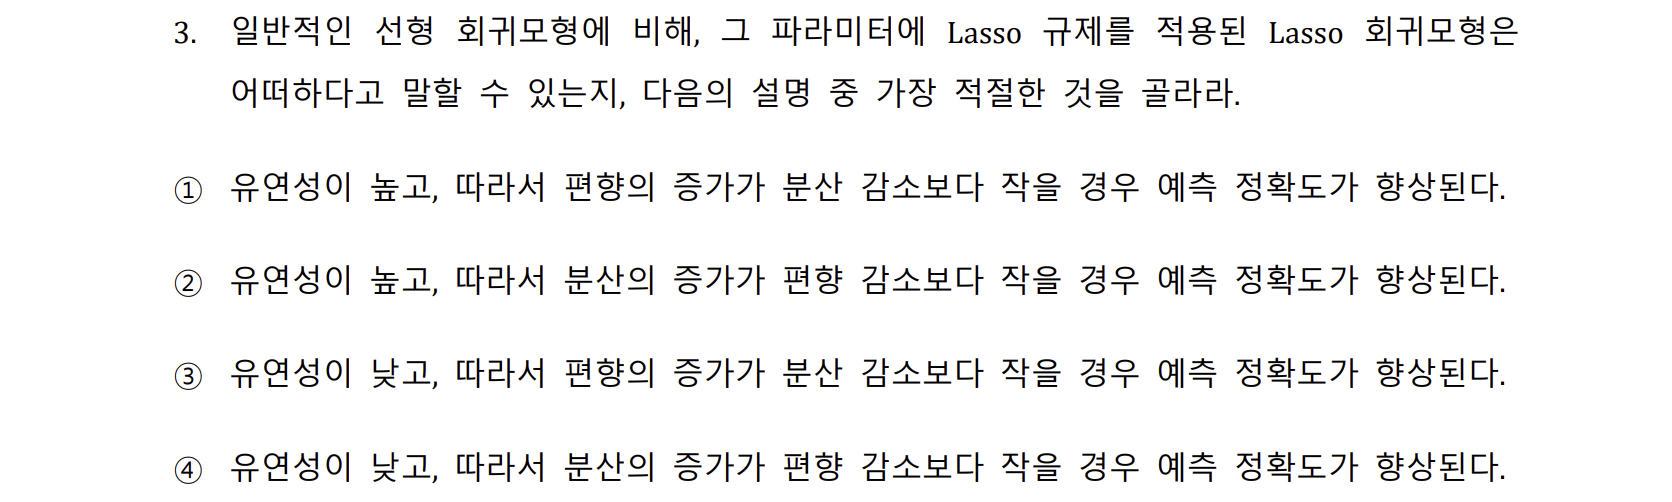
\includegraphics{image/machine_hw1_4.png}

\subsubsection{Answer : 3번}\label{answer-3uxbc88}

\textbf{기본적으로 규제가 있는 회귀모형은 일반적인 회귀모형에 비하여
유연성이 떨어집니다.}

비용함수를 최소화시켜나가는 과정에서 파라미터가 만족해야할 추가적인
조건이 붙기 때문입니다.

이를 알기 쉽게 경사하강법을 예시로 들어보면, 매 파라미터를
업데이트해나갈 때,

\textbf{규제가 있는 회귀모형에서는 규제로 인해 업데이트를 원하는 만큼
실시할 수 없게} 됩니다.

따라서 규제가 조금이라도 존재한다면, 일반적인 회귀모형에 비해서 유연성이
떨어집니다.

\textbf{유연성은 떨어지는 대신 장점이 있는데, 모델의 overfitting 문제를
잘 해결}한다는 것 입니다.

모델이 train data로 훈련할 때 파라미터에 제약을 가하기 때문에, 모델이
과적합되지 않도록 적정히 조절하게 됩니다.

\textbf{이를 종합해보면, 규제가 있는 회귀모형은 유연성이 떨어져 다소
편향이 발생하게 되지만,}

\textbf{과적합을 방지함으로써 분산이 감소되는 효과 있다는 의미}가
됩니다.

따라서 규제의 여부와 규제의 정도를 결정할 때, 이러한 trade-off를 잘
이해하여야 합니다.

\textbf{분산 감소효과가 편향 증가효과보다 클 때, 규제를 가하거나 규제의
정도를 강화하는 것이 적합}할 것 입니다. \textbf{\emph{(3번)}}



\end{document}
